\begin{frame}{¿Qué es Git?}
  \begin{columns}[onlytextwidth]
    \column{0.5\textwidth}
    \begin{center}
      
\includegraphics[scale=0.07]{images/logoGit2}
    \end{center}
    \column{0.5\textwidth}
    Git es un Sistema de Control de Versiones (VCS) que nos permite gestionar los cambios que realizamos un proyecto.
  \end{columns}
\end{frame}

\begin{frame}{¿Qué es Git?}
  \begin{columns}[onlytextwidth]
    \column{0.5\textwidth}
    \alert{\Large ¿Git = GitHub? {\color{solarized-red} \textbf{No}}} \\
    GitHub es una forja (plataforma de desarrollo colaborativo) para alojar proyectos Git.
    \column{0.5\textwidth}
    \begin{center}
      \animategraphics[height=1.3in,autoplay,loop] {12}{images/DF/githubDP1_}{0}{7}
      \animategraphics[height=1.3in,autoplay,loop] {12}{images/DF/githubDP2_}{0}{13}
    \end{center}
  \end{columns}
\end{frame}

\begin{frame}{¿Qué es Git?}
  \alert{\Large ¿Cómo se utiliza Git?}
  \begin{columns}[onlytextwidth]
    \column{0.6\textwidth}
    Git se utiliza mediante comandos en la \textbf{Terminal}. \\

    Pero existen:
    \begin{itemize}
      \item Clientes gráficos (GitKraken, SourceTree, GitHub Desktop...)
      \item Integración en muchos editores e IDEs (Atom, Visual Studio Code, Eclipse...)
    \end{itemize}
    \vspace{0.5cm}
    \uncover<2>{
    {\color{violet}\large Lo mejor es la \textbf{Terminal}.}}
    \column{0.4\textwidth}
    \uncover<2>{
    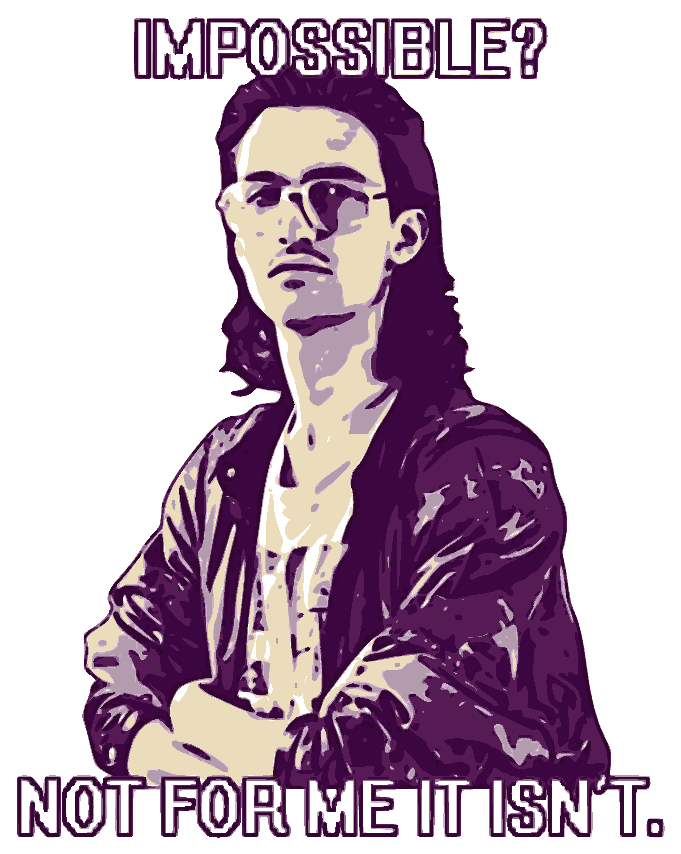
\includegraphics[scale=0.4]{images/hackerMan.eps}}
  \end{columns}
\end{frame}
